\ifdefined\COMPLETE
\else
\documentclass[11pt]{article}
\usepackage[french, english]{babel}
\usepackage[utf8]{inputenc}
\usepackage{graphicx}
\usepackage{framed}
\usepackage[normalem]{ulem}
\usepackage{amsmath}
\usepackage{amsthm}
\usepackage{amssymb}
\usepackage{amsfonts}
\usepackage{enumerate}
\usepackage{import}
\usepackage[top=1 in,bottom=1in, left=1 in, right=1 in]{geometry}
\usepackage{listingsutf8}
\usepackage{color}
\usepackage{float}
\usepackage{graphicx}
\usepackage{subcaption}
\usepackage[toc,page]{appendix}
\usepackage{multicol}
\usepackage{wrapfig}
\usepackage{sidecap}

\floatstyle{boxed} 
\restylefloat{figure}
\definecolor{mygreen}{rgb}{0,0.6,0}
\definecolor{mygray}{rgb}{0.5,0.5,0.5}
\definecolor{mymauve}{rgb}{0.58,0,0.82}
\newcommand{\dt}{\partial_t}
\newcommand{\Tl}{\frac{T}{\lambda}}
\theoremstyle{definition}
\newtheorem{definition}{Définition}[section]
\DeclareMathOperator*{\argmax}{arg\,max}
\DeclareMathOperator*{\argmin}{arg\,min}
 


\lstset{ 
  backgroundcolor=\color{white},   % choose the background color; you must add \usepackage{color} or \usepackage{xcolor}; should come as last argument
  basicstyle=\footnotesize,        % the size of the fonts that are used for the code
  breakatwhitespace=false,         % sets if automatic breaks should only happen at whitespace
  breaklines=true,                 % sets automatic line breaking
  captionpos=b,                    % sets the caption-position to bottom
  commentstyle=\color{mygreen},    % comment style
  deletekeywords={...},            % if you want to delete keywords from the given language
  escapeinside={\%*}{*)},          % if you want to add LaTeX within your code
  extendedchars=true,              % lets you use non-ASCII characters; for 8-bits encodings only, does not work with UTF-8
  firstnumber=1000,                % start line enumeration with line 1000
  frame=single,	                   % adds a frame around the code
  keepspaces=true,                 % keeps spaces in text, useful for keeping indentation of code (possibly needs columns=flexible)
  keywordstyle=\color{blue},       % keyword style
  language=Python,                 % the language of the code
  morekeywords={*,...},            % if you want to add more keywords to the set
  numbers=left,                    % where to put the line-numbers; possible values are (none, left, right)
  numbersep=5pt,                   % how far the line-numbers are from the code
  numberstyle=\tiny\color{mygray}, % the style that is used for the line-numbers
  rulecolor=\color{black},         % if not set, the frame-color may be changed on line-breaks within not-black text (e.g. comments (green here))
  showspaces=false,                % show spaces everywhere adding particular underscores; it overrides 'showstringspaces'
  showstringspaces=false,          % underline spaces within strings only
  showtabs=false,                  % show tabs within strings adding particular underscores
  stepnumber=2,                    % the step between two line-numbers. If it's 1, each line will be numbered
  stringstyle=\color{mymauve},     % string literal style
  tabsize=2,	                   % sets default tabsize to 2 spaces
  title=\lstname                   % show the filename of files included with \lstinputlisting; also try caption instead of title
}
\lstset{inputencoding=utf8/latin1}
\newcommand{\Dt}{\Delta t}
\newcommand{\Dx}{\Delta x}
 %file containing all the used libraries
\begin{document}
\fi

\section{Schémas Numériques}
On a le modèle suivant (``KPP avec mémoire"): 
\begin{equation} \left\{
                \begin{array}{ll}
                   \dt\mu = K\Delta\mu + C(\mu + \rho) -\mu\rho\\
                 \dt\rho=  F_0 \mu \\
                  \dt C = -b\rho C
                \end{array}
              \right.
\end{equation}
\subsection{Pour l'équation différentielle ordinaire}
Sans dépendance spatiale:
\begin{equation} \left\{
                \begin{array}{ll}
                   \dt\mu = C(\mu + \rho) -\mu\rho\\
                 \dt\rho=  F_0 \mu \\
                  \dt C = -b\rho C
                \end{array}
              \right.
\end{equation} 
\subsubsection{Schéma semi-implicite I pour l'EDO}
Soit le schéma semi-implicite I pour l'EDO:
\begin{equation} \boxed{\left\{
                \begin{array}{ll}
                   \mu^{n+1} = \mu^{n}+  \Dt( C^{n}(\mu^{n+1} + \rho^{n+1}) -\mu^{n+1}\rho^{n})\\
                \rho^{n+1}=  \rho^{n}+ \Dt (F_0 \mu^{n+1}) \\
                 C^{n+1} =C^{n}- \Dt(b\rho^{n+1}C^{n+1})
                \end{array}
              \right.}
\end{equation}
Ce schéma donne:
\begin{equation*} \left\{
                \begin{array}{ll}
                   \mu^{n+1}(1-\Dt(C^{n}(1+\Dt F_0)) + \rho^{n}) = \mu^{n}+  \Dt C^{n}\rho^{n} \\
                \rho^{n+1}=  \rho^{n}+ \Dt (F_0 \mu^{n+1}) \\
                 C^{n+1} =C^{n}\frac{1}{1+ \Dt b\rho^{n+1}}
                \end{array}
              \right.
\end{equation*}
\paragraph{Positivité du schéma}
Pour conserver la positivité il suffit que le terme $(1-\Dt(C^{n}(1+\Dt F_0)) + \rho^{n}) $ reste positif:\\
Par exemple: 
\begin{equation}
	\boxed{C^0< \frac{1}{\Dt(1+F_0\Dt)}}
\end{equation}

\subsubsection{Schéma semi-implicite II pour l'EDO}
Soit le schéma semi-implicite II pour l'EDO:
\begin{equation} \boxed{\left\{
                \begin{array}{ll}
                   \mu^{n+1} = \mu^{n}+  \Dt( C^{n}(\mu^{n+1} + \rho^{n+1}) -\mu^{n}\rho^{n})\\
                \rho^{n+1}=  \rho^{n}+ \Dt (F_0 \mu^{n+1}) \\
                 C^{n+1} =C^{n}- \Dt(b\rho^{n+1}C^{n+1})
                \end{array}
              \right.}
\end{equation}
Ce schéma donne:
\begin{equation*} \left\{
                \begin{array}{ll}
                   \mu^{n+1}(1-\Dt(C^{n}(1+\Dt F_0))) = \mu^{n}+  \Dt \rho^{n}(C^{n}-\mu^{n}) \\
                \rho^{n+1}=  \rho^{n}+ \Dt (F_0 \mu^{n+1}) \\
                 C^{n+1} =C^{n}\frac{1}{1+ \Dt b\rho^{n+1}}
                \end{array}
              \right.
\end{equation*}
\paragraph{Positivité du schéma}
Pour conserver la positivité il suffit que les terme $(1-\Dt(C^{n}(1+\Dt F_0)))$ et $\mu^{n}+  \Dt \rho^{n}(C^{n}-\mu^{n})$ restent positif:\\
Par exemple: 
\begin{equation}
	\boxed{C^0< \frac{1}{\Dt(1+F_0\Dt)}}
\end{equation}
et 
\begin{equation}
	\boxed{\rho^n< \frac{1}{\Dt}}
\end{equation}
On obtient une condition de plus que le schéma semi-implicite I.
\subsection{Pour l'équation aux dérivées partielles}
\subsubsection{Schéma semi-implicite I pour l'EDP en 1D}
Soit le schéma semi-implicite I pour l'EDP en 1D:
\begin{equation} \boxed{\left\{
                \begin{array}{ll}
                   \mu^{n+1}_i = \mu^{n}_i+ K\Dt \frac{\mu^{n+1}_{i+1}-2\mu^{n+1}_i+\mu^{n+1}_{i-1}}{\Dx ^2} + \Dt( C^{n}_i(\mu^{n+1}_i + \rho^{n+1}_i) -\mu^{n+1}_i\rho^{n}_i)\\
                \rho^{n+1}_i=  \rho^{n}_i+ \Dt (F_0 \mu^{n+1}_i) \\
                 C^{n+1}_i =C^{n}_i- \Dt(b\rho^{n+1}_iC^{n+1}_i)
                \end{array}
              \right.}
\end{equation}
Ce schéma a été construit pour donner une équation linéaire en $\mu^{n+1}$:
\begin{equation*} \left\{
                \begin{array}{ll}
                   (1+\frac{K\Dt}{\Dx^2}A-\Dt(C^{n}(1+\Dt F_0)) + \rho^{n})\mu^{n+1} = \mu^{n}+  \Dt C^{n}\rho^{n} \\
                \rho^{n+1}=  \rho^{n}+ \Dt (F_0 \mu^{n+1}) \\
                 C^{n+1} = C^{n}\frac{1}{1+ \Dt b\rho^{n+1}}
                \end{array}
              \right.
\end{equation*}
où $A$ est la matrice de discrétisation par différences finies de $-\Delta$ en 1D
:\begin{equation}  \label{myeq}A= \left[ \begin{matrix}2 & -1 & & 0\\-1 & \ddots & \ddots &  \\& \ddots & \ddots &  -1 \\0 &  & -1 & 2  \end{matrix}  \right]\end{equation}
Remarque: pour le schéma en dimension $n\geq 2$, il suffit de remplacer $A$ par la matrice de discrétisation par différences finies de $-\Delta$ en dimension $n$.
\paragraph{Positivité du schéma:}
Afin de préserver la positivité, on obtient la même condition (suffisante) que pour l'EDO:
\begin{equation}
	\boxed{C^0< \frac{1}{\Dt(1+F_0\Dt)}}
\end{equation}
\begin{proof} Supposons $\mu^0 >0$.\\ Raisonnons par l'absurde et supposons que $n=\min{n \mid \exists j \mid \mu^{n+1}_j < 0}$ existe. Soit $j = \argmin{\mu^{n+1}_i}$.\\
On a $(1-\Dt(C^{n}_j(1+\Dt F_0)) + \rho^{n}_j)\mu^{n+1}_j = \mu^{n}+  \Dt C^{n} +\frac{K\Dt}{\Dx^2}(\mu^{n+1}_{j+1} - 2\mu^{n+1}_j + \mu^{n+1}_{j-1}) $. \\
Or par définition de $n$ et comme $C^0< \frac{1}{\Dt(1+F_0\Dt)}$ et $C^n < C^0$:\\
 Donc $ \mu^{n}+  \Dt C^{n} > 0$ et
 $ 1-\Dt(C^{n}_j(1+\Dt F_0)) + \rho^{n}_j > 0$. \\
Et par définition de $j$: 
$\mu^{n+1}_{j+1} - 2\mu^{n+1}_j + \mu^{n+1}_{j-1} \geq 0$.\\
On a donc $\mu^{n+1}_j > 0$ mais   $\mu^{n+1}_j = \min(\mu^{n+1}_i) < 0$ par définition de $j$ et $n$ : C'est absurde.
\end{proof}

\newpage
\section{Résolution numérique}
\subsection{Résolution de l'EDO}
\subsubsection{Résultat de la simulation de l'EDO}
\begin{figure}[hbt!]
\centering
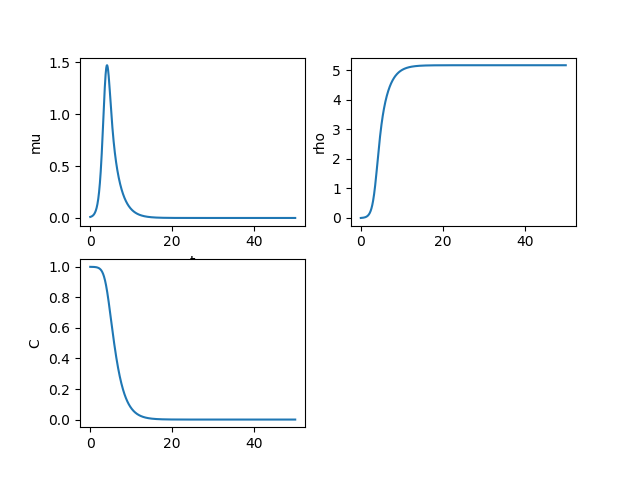
\includegraphics[width=.9\textwidth]{Images/edo_euler_implicite.png}
\caption{Résolution du schéma implicite pour l'EDO}
\end{figure}

\subsubsection{Observations de la simulation de l'EDO}
 On observe les phénomènes attendus sur l'EDO:\\
 -i) $\mu$ est bornée et tend vers 0.\\
 -ii) $\rho$ est croissante et bornée.\\
 -iii) $C$ décroît vers 0.
 \newpage
 -iv) Les solutions ont un comportement exponentiel autour des états stationnaires et ce comportement est bien prédit par la linéarisation de l'EDO autour de ces états:

\begin{SCfigure}[][h]
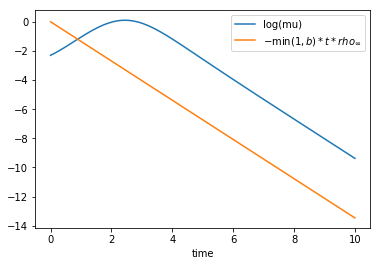
\includegraphics[width=0.4\textwidth]{Images/linearisation.png}
\caption{Comportement de $\log(\mu)$, en particulier autour de $(\mu,\rho,C) =  (0,\rho_\infty,0)$. $\log(\mu)$ est bien linéaire autour des états stationnaires et sa pente (le facteur dans l'exponentielle) correspond exactement à $-\min(1,b)\rho_\infty$ ce qui est un résultat obtenu dans la partie Linéarisation } 
\end{SCfigure} 
 
 -v) L'ordre de convergence de l'EDO observé est de 1:
\begin{SCfigure}[][h]
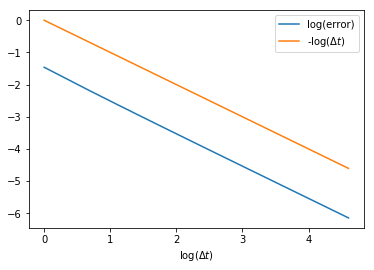
\includegraphics[width=0.4\textwidth]{Images/ordrecvedo.png}
\caption{Comportement du $\log(erreur)$ quand $\Delta t   0$. La solution du schéma semi implicite I est comparée à différents pas de temps $\Delta t$ à la solution numérique du schéma de Runge-Kutta avec $\Delta t = 2*10^{-7}$. On observe bien que la convergence est d'ordre 1.}
\end{SCfigure} 

\newpage
\subsection{Résolution de l'EDP en 1D}
\subsubsection{Résultat de la simulation de l'EDP en 1D}
\begin{figure}[hbt!]
\centering
\begin{subfigure}[b]{0.45\textwidth}
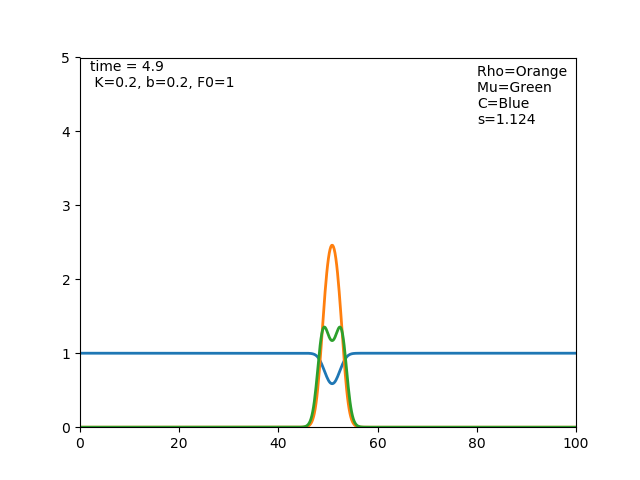
\includegraphics[width=\textwidth]{Images/edp_1d_0.png}
\end{subfigure}
\begin{subfigure}[b]{0.45\textwidth}
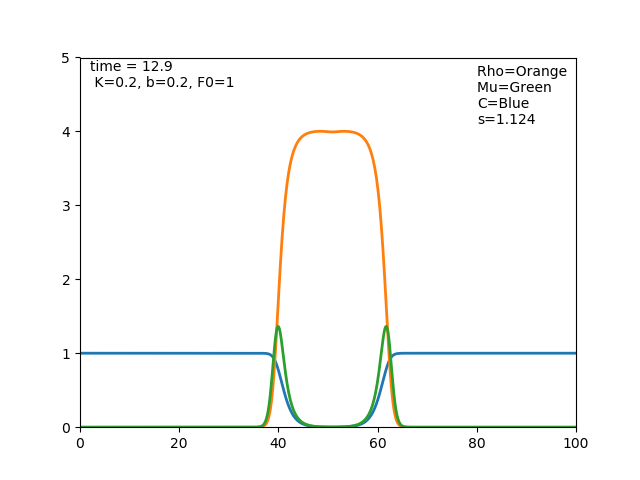
\includegraphics[width=\textwidth]{Images/edp_1d_1.png}
\end{subfigure}
\begin{subfigure}[b]{0.45\textwidth}
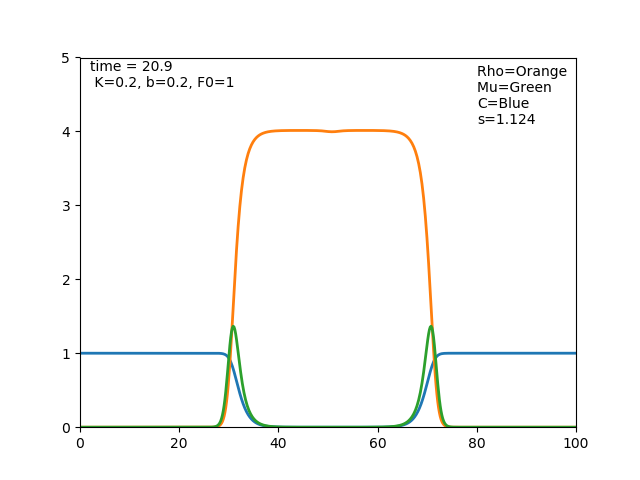
\includegraphics[width=\textwidth]{Images/edp_1d_2.png}
\end{subfigure}
\begin{subfigure}[b]{0.45\textwidth}
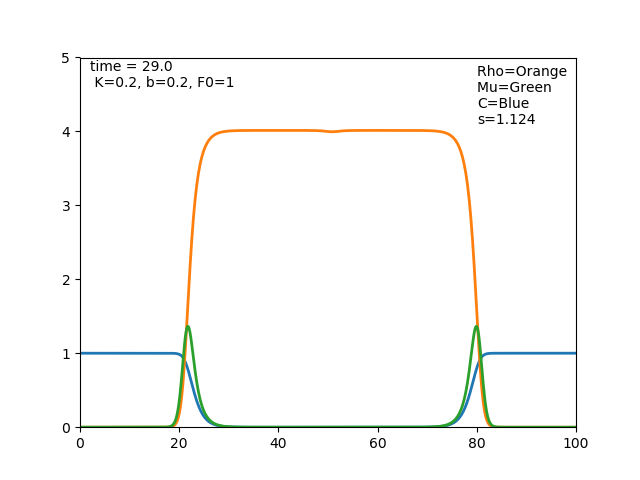
\includegraphics[width=\textwidth]{Images/edp_1d_3.png}
\end{subfigure}
\caption{Résolution du schéma semi implicite I pour l'EDP en 1D} 
\end{figure}
On voit sur les simulations que la solution tend vers une solution de type onde plane stationnaire. Il est possible de calculer cette vitesse et de la comparer avec la vitesse théorique minimale obtenue dans la partie 3: 

\newpage
 
\begin{figure}[hbt!]
\centering
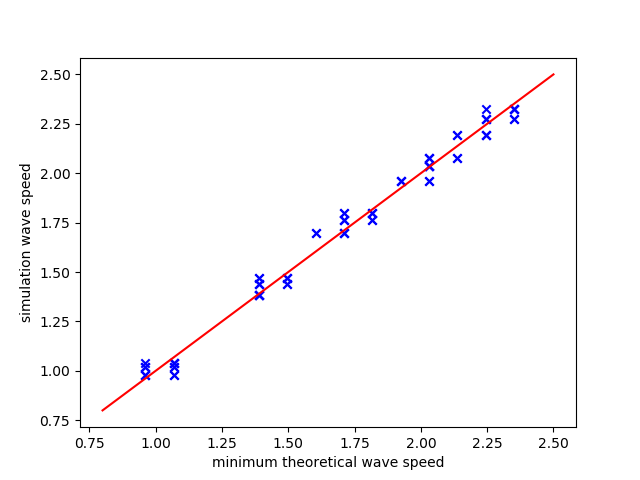
\includegraphics[width=.7\textwidth]{Images/stheoriquevssimulations.png}
\caption{Vitesse du front observée numériquement en fonction de la vitesse minimale théorique}
\end{figure}
Soit \begin{equation*}
s^*_{theorique} =K\frac{f_0(18F_0+4)+\sqrt{f_0(f_0(18F_0+4)^2+108(f_0+4F_0)F_0^2)}}{2(f_0+4F_0)}\end{equation*} la vitesse minimale théorique obtenue dans la partie 3.\\
Ce graphe représente par les points bleus la vitesse du front observée numériquement pour différentes simulations en fonction de la vitesse minimale théorique associée à cette simulation. La droite rouge est la droite $s_{simu} = s^*_{theorique}$.\\
On remarque que la vitesse du front observée numériquement est très proche de la vitesse minimale théorique: ce phénomène est similaire à celui de l'équation de Fisher-KPP: pour une donnée initiale à support compact, \textbf{le front se propage asymptotiquement à la vitesse minimale de l'équation d'onde associée à l'EDP}.


\newpage
\subsection{Résolution de l'EDP en 2D}

\begin{figure}[hbt!]
\centering
\begin{subfigure}[b]{\textwidth}
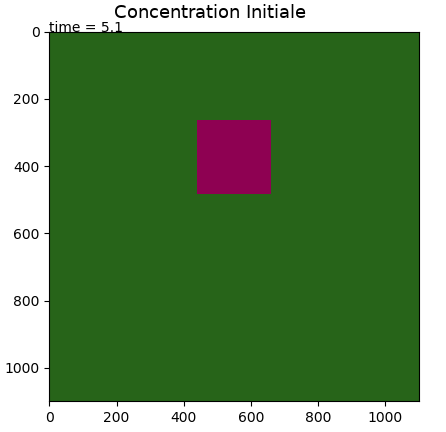
\includegraphics[width=.35\textwidth]{Images/CInitial.png}
\end{subfigure}
\begin{subfigure}[b]{0.45\textwidth}
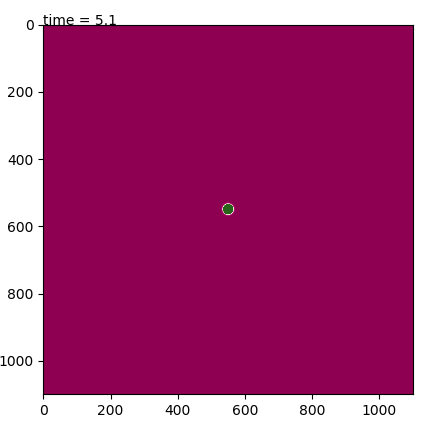
\includegraphics[width=\textwidth]{Images/Rho2d0.png}
\end{subfigure}
\begin{subfigure}[b]{0.45\textwidth}
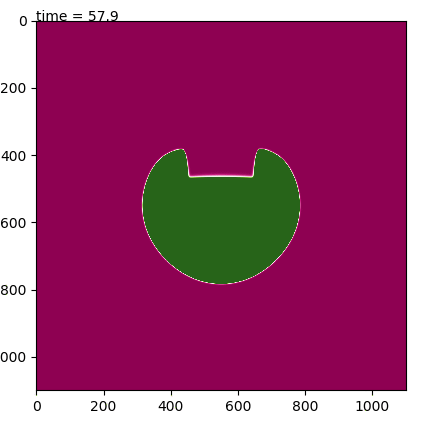
\includegraphics[width=\textwidth]{Images/rho2d1.png}
\end{subfigure}
\begin{subfigure}[b]{0.45\textwidth}
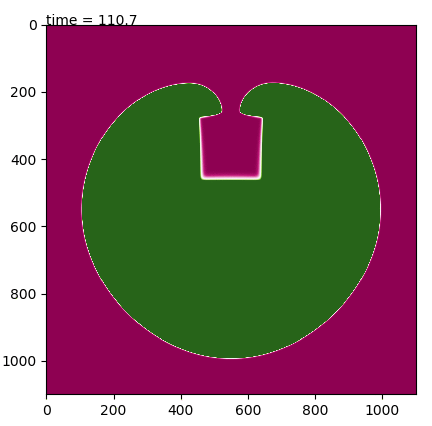
\includegraphics[width=\textwidth]{Images/rho2d2.png}
\end{subfigure}
\begin{subfigure}[b]{0.45\textwidth}
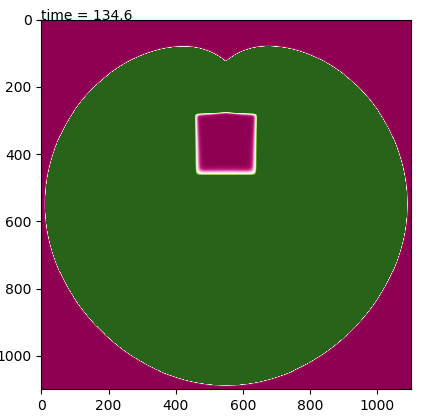
\includegraphics[width=\textwidth]{Images/rho2d3.png}
\end{subfigure}
\caption{Évolution de $\rho$ pour la résolution du schéma semi implicite I pour l'EDP en 2D avec un trou de concentration. Ici la grille est de taille 1100x100, avec 1000 pas de temps.} 
\end{figure}
\newpage
Deux challenges numériques ont étés rencontrés:
\begin{paragraph}
- 1) Temps d’exécution: le schéma consiste principalement à résoudre à chaque pas de temps une équation matricielle $AX=B$, où $A$ est de taille $n = 1100*1100= 1.21*10^6$. Une idée naive serait alors de calculer $A^{-1}$ par exemple par pivot de gauss, qui a un coup $\mathcal{O}(n^3)$, ou par l'algorithme de Strassen qui est un peu plus efficace $\mathcal{O}(n^{2.8})$. Cependant ces stratégies ne sont pas efficaces car il n'est pas nécessaire de calculer l'inverse de $A$: On cherche seulement l'antécédent d'une image. La stratégie implémentée ici est de trouver $X$ par méthode des minimums résiduels, c'est à dire minimiser la fonction $x\to || Ax-B||^2 $ par méthode des moindres carrées, méthode qui fonctionne pour les matrices symétriques et qui est très rapide pour les matrices creuses (notre cas).\\ On peut encore accélérer la convergence de la méthode des minimums résiduels en précisant pour $\mu^{n+1}$ le guess $\mu^n$ et en conditionnant le système par la matrice Identité. \end{paragraph}
\begin{paragraph}
- 2) Coup en mémoire: Une matrice carrée de taille $1.21*10^6$ pèse 10GB de RAM sous Python... Heureusement, dans notre cas la matrice A est creuse et il existe des méthodes et librairies adaptées pour représenter de telles matrices efficacement. De plus chaque $\rho^n,\mu^n$ et $C^n$ est représenté par une matrice carrée de taille $1100$, ce qui pèse 10MB. Ces matrices ne sont pas creuses donc il est plus dur de les compresser. Si l'on veut stocker ces quantités pour ensuite retracer l’évolution de $\rho,\mu,C$ pour 1000 pas de temps, ceci coûterait 30GB de RAM... Il faut donc faire des compromis.
\end{paragraph}
\ifdefined\COMPLETE
\else
\end{document}
\fi